\documentclass{article}
\usepackage[utf8]{inputenc}
\usepackage{natbib}           % Bibliography
\usepackage{graphicx}         % Tables and figures
\usepackage{threeparttable}   % Table and figure notes: \tablenotes{}

\title{My First Project}
\author{}
\date{}

\begin{document}

\maketitle

% ============================== CHAPTER 1 ============================== %
\section{My First Chapter}
This chapter displays my first table, Table~\ref{tab:myfirsttable}, and my first figure, Figure~\ref{fig:myfirstfigure}. They are based on Stata's auto dataset, see \citet{stata_press_datasets_2021}.

% My First Table
\begin{table}[!ht]
\caption{My First Table}
\label{tab:myfirsttable}
\centering
	{
\def\sym#1{\ifmmode^{#1}\else\(^{#1}\)\fi}
\begin{tabular}{l*{1}{cccc}}
\hline\hline
                    &        mean&          sd&         min&         max\\
\hline
Price               &    6146.043&     2912.44&        3291&       15906\\
Mileage (mpg)       &    21.28986&    5.866408&          12&          41\\
Repair Record in 1978&    3.405797&    .9899323&           1&           5\\
Foreign             &    1.304348&    .4635016&           1&           2\\
\hline
Observations        &          69&            &            &            \\
\hline\hline
\end{tabular}
}

\begin{tablenotes}
	\item \emph{Notes:} The table shows summary statistics for selected variables.
\end{tablenotes}
\end{table}

% My First Figure
\begin{figure}[!ht]
\caption{My First Figure}
\label{fig:myfirstfigure}
\centering
	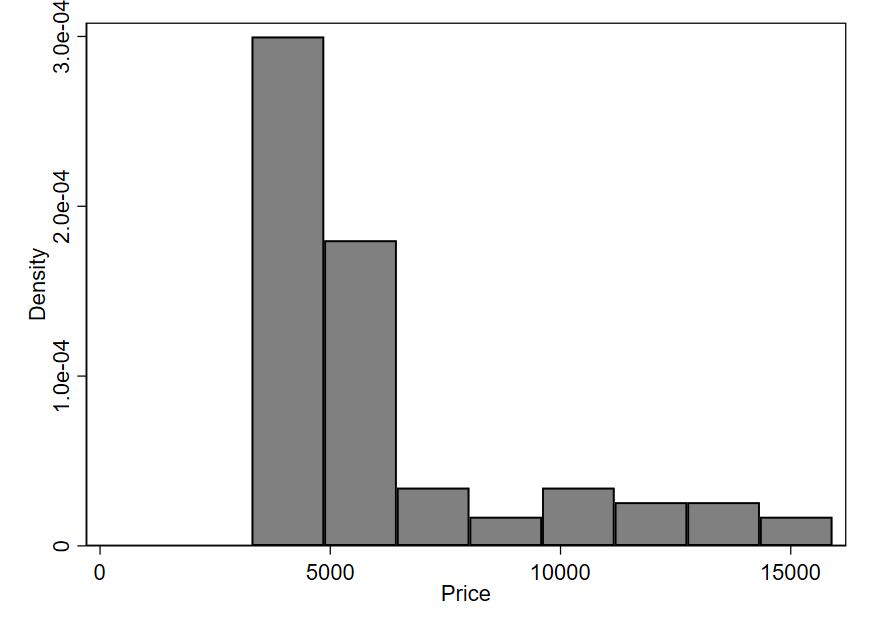
\includegraphics[width=0.75\textwidth]{../output/figures/myfirstfigure.png}
\begin{tablenotes}
	\item \emph{Notes:} The figure shows the distribution of prices.
\end{tablenotes}
\end{figure}


% ============================== BIBLIOGRAPHY ============================== %
\bibliographystyle{aer}
\bibliography{../literature/bibliography.bib}

\end{document}
